%Introduction to LaTeX
% !TeX root = ../thesis.tex

\chapter{BaMa Template}

\section{\LaTeX~Basics}

LaTeX uses source code which is compiled to generate documents. This has several advantages when creating large documents: 

\begin{itemize}
	\item Separation of template and document possible
	\item Consistent text format across sections and documents oriented at norms like DIN~1450
	\item Customisable and reproducible generation of table of contents, figures and index
	\item Automation of tasks like number formatting, plot generation, \dots
	\item Inclusion of external files like measurement data without the need for copy and paste
	\item Automated tasks like number formatting 
\end{itemize}

\subsection{Command syntax}

LaTeX commands have the following syntax:

\begin{lstlisting}
	\command[options]{argument}
\end{lstlisting}

There are also environments which can be opened and closed:

\begin{lstlisting}
	\begin{environmentname}
		...
	\end{environmentname}
\end{lstlisting}

As the backslash is used as prefix for commands and the percent sign for commands a few escape sequences are necessary as listed in table~\ref{tab:escseq}. For more special characters see \url{http://detexify.kirelabs.org/classify.html}.

\begin{table}[H]
	\centering
	\caption{\LaTeX escape sequences}
	\label{tab:escseq}
	\begin{tabular}{ccc}
		\toprule
		Sign & \LaTeX special meaning  & Escape sequence\\
		\midrule
		\textbackslash~(backslash) & command initializer & \verb|\textbackslash| \\
		\%~(percent) & comment for rest of line & \verb|\%| \\
		\textasciitilde~(tilde) & line break protected space & \verb|\textasciitilde| \\
		\$~(dollar sign) & start math mode & \verb|\$| \\			
		\bottomrule
	\end{tabular}
\end{table}

\subsection{Main document structure}

Documents normally have the following components:

\begin{itemize}
	\item \verb|\documentclass[options]{classname}|: Loads the documents template which defines the appearance like article, conference paper, \dots. The bama template uses a custom class located in the main directory of the repository.
	\item \verb|\usepackage[options]{packagename}|: Loads packages for additional capabilities. More information about packages is available at ctan \footnote{\url{https://www.ctan.org/}}.
	\item \verb|\input{filename}|: Inserts the content of another \TeX file \footnote{include serves a similar purpose, has more restrictions but offers  higher compilation speeds.}.
	\item The content of the document in between \verb|\begin{document}| and \verb|\end{document}|
\end{itemize}

\subsection{Heading structure}

There are several levels of headings which are listed in the following. Avoid having a single heading of a certain hierarchy e.g. if there is section 1.1 there should also be at least 1.2.

\begin{description}
	\item [part] is the highest hierarchy. Parts have big headings occupying a whole page. It is not needed for the thesis.
	\item [chapter] is a high hierarchy heading causing page breaks to next uneven page. It is not available in all classes but should be used for the thesis.
	\item [section] is used to separate chapters. One can also use \verb|\subsection| and \verb|\subsubsection| for further hierarchy levels.
	\item [paragraph] and \verb|\subparagraph| are used for small passages and do not cause a line break after the heading.
\end{description}

\subsection{Text formatting}

LaTeX distinguishes between line break and paragraph. Do not use the line break operator for paragraphs, just insert an empty line in the source code. Sometimes special formatting is useful e.g. to center figures but manual font size and style changes in normal text should be avoided.

\begin{table}[H]
	\centering
	\caption{Text formatting}
	\label{tab:textformat}
	\begin{tabular}{ccc}
		\toprule
		Feature & command\\
		\midrule
		Line break & \verb|\\| \\
		Paragraph & empty line in code \\
		\textit{italic} & \verb|\textit{...}| \\
		\textbf{bold} & \verb|\textbf{...}| \\
		center & \verb|\centering| \\	
		\bottomrule
	\end{tabular}
\end{table}

\subsection{Dashes}

\begin{table}[H]
	\centering
	\caption{Dashes}
	\label{tab:dashes}
	\begin{tabular}{cccc}
		\toprule
		Name & Code & Example & Usage\\
		\midrule
		dash & \verb|-| & - & hyphen\\
		Viertelgeviertstrich & &  & Binde-, Trennungs-, Ergänzungsstrich\\
		en dash & \verb|--| & -- & number range\\
		Halbgeviertstrich & & & Gedanken-, Bis-strich, bei Geldbeträgen\\
		em dash & \verb|---| & --- & parenthetic expression \\
		Geviertstrich &  & & Spiegelstrich\\
		%Doppelgeviertstrich & \verb|--\,--| & --\,-- & Zensurstrich (englisch)
		\bottomrule
	\end{tabular}
\end{table}

Hyphens are automatically inserted to break lines and achieve justification. Although the corresponding parameters should be set correctly special words can lead to problems. For example MUSIC-Alogrithmus has a dash which means that hypens at other places are not allowed. This can be prevented by the syntax \hbox{\verb|MUSIC-Algo\-rithmus|} which allows an optional line break. The same problems can occur due to protected whitespaces.

\subsection{Lists}

There are two major list types in {\LaTeX}: numerated (\texttt{enumerate}) and not numerated (\texttt{itemize}). Furthermore there is the type \texttt{description} for explaining keywords. Lists are started with \texttt{begin} and stopped with \texttt{end}. They can also be nested.

\begin{enumerate}
	\item High level with numbering
	\begin{itemize}
		\item Detailed information
		\item without numeration
	\end{itemize}
	\item Another big point
	\item \dots and more
\end{enumerate}

\begin{lstlisting}[language=TeX]
\begin{enumerate}
	\item High level with numbering
	\begin{itemize}
		\item Detailed information
		\item without numeration
	\end{itemize}
	\item Another big point
	\item \dots and more
\end{enumerate}
\end{lstlisting}

\section{Math mode and Numbers}

	Normaly LaTeX operates in text mode, but for expressions like $x=5$ the math mode can be activated and deactivated using \verb|$|. In math mode text is italic and exhibits changed letter spacing.
	
	For indexed equations the \verb|equation| environment is suited when using vanilla LaTeX. With the package \verb|amsmath| the \verb|align| environment is available which is recommended here:
	
	\begin{align}
		\label{eq:alignDemo}
		\oint_{\partial A} \vect{B}_\text{ind} \dd{\vect{l}} &= \mu_0 \left( \iint_A \vect{j}_\text{ind} \dd{\vect{A}} + \varepsilon_0 \frac{\partial}{\partial t} \iint_A \vect{E} \dd{\vect{A}} \right) \\
		\text{und außerdem} \nonumber \\
		\label{eq:alignDemo2}
		Q &= \oiint_A \vect{D} \dd{\vect{A}} = \iiint_V \rho_{\text{Volumen}} \dd{V}
	\end{align}
	
	\begin{lstlisting}[language=TeX]
	\begin{align}
	\label{eq:alignDemo}
	\oint_{\partial A} \vv*{B}{\text{ind}} \dd{\vv{l}} &=
		\mu_0 \left( \iint_A \vv*{j}{\text{ind}} \dd{\vv{A}}
		+ \varepsilon_0 \frac{\partial}{\partial t} \iint_A \vv{E} \dd{\vv{A}} \right) \\
	\text{und außerdem} \nonumber \\
	\label{eq:alignDemo2}
	Q &= \oiint_A \vv{D} \dd{\vv{A}} = \iiint_V \rho_{\text{Volumen}} \dd{V}
	\end{align}
	\end{lstlisting}

	Equations can be easily referenced when the package \verb|mathtools| is used by the the command \verb|\eqref{eq:alignDemo}| (e.g. Eq.~\eqref{eq:alignDemo}).
	
	Between numbers and units a half length space has to be inserted (\verb|\,|) \footnote{For details see DIN~1338}. In German a comma has to be used instead of a dot. The package \verb|siunitx| can handle the correct formatting of numbers with units. The syntax is showed in table~\ref{tab:numberUnitFormat}. Also note that in German the letter \enquote{$U$} is used for voltage instead of \enquote{$V$}.
	
	\begin{table}
		\centering
		\caption{Number- and Unit formatting}
		\label{tab:numberUnitFormat}
		\begin{longtable}{p{.25\textwidth}p{.1\textwidth}p{.1\textwidth}p{.4\textwidth}}
			\toprule
			Variables & \textit{italic} & $x$\newline $y$\newline $f$\newline $\omega$ & \verb|$x$|\newline \verb|$y$|\newline \verb|$f$|\newline \verb|$\omega$|\\
			Scientific constants & \textit{italic} & $c_0$\newline $\mu_0$\newline $\varepsilon_0$ & \verb|$c_0$|\newline \verb|$\mu_0$|\newline \verb|$\varepsilon_0$|\\
			Units & upright & \si{\milli\ampere}\newline $\SI{3.0}{\micro\metre}$\newline \SI{1.41}{} & \verb|\si{\milli\ampere}|\newline \verb|$\SI{3.0}{\micro\metre}$|\newline \verb|\SI{1.41}{}|\\
			Operators & upright & $\frac{\dd{x}}{\dd{y}}$\newline $\sin$\newline $\cos$\newline $\arg$ & \verb|$\frac{\dd{x}}{\dd{y}}$|\newline \verb|$\sin$|\newline \verb|$\cos$|\newline \verb|$\arg$|\\
			Mathematic constants & upright & $\ee$\newline $\ii$\newline $\jj$\newline $\pipi$ & \verb|$\ee$|\newline \verb|$\ii$|\newline \verb|$\jj$|\newline \verb|$\pipi$| \\
			\bottomrule
		\end{longtable}
	\end{table}

	\section{Floating environments}
	\label{sec:floatenvironments}
	
		Floating objects are objects whose position in the final document can depart from the source code. The most common floating objects are figures and tables. Commonly they are placed at the top or bottom of a page to not split the text apart and make reading more pleasant. Floats can also be longer than a single page.
		
		Floats are created by using \verb|\begin{figure}| / \verb|\end{figure}| for figures and \verb|\begin{table}| / \verb|\end{table}| for tables. The content is defined in between and can be arbitrarily chosen. Floats should have a meaningful caption which is specified with \texttt{{\textbackslash}caption[register entry]\{caption text\}}. The command \texttt{{\textbackslash}label} is used to enable referencing them.
		
		Sometimes {\LaTeX} has troubles to determine the best position for a float. In these cases optional arguments or packages like \texttt{placeins} can be used.
		
		\begin{itemize}
			\item t (top, top of page)
			\item b (bottom, bottom of page)
			\item p (page, on an individual page)
			\item h (here, exactly at this position)
			\item H (HERE, forced to place exactly at this position (provided by the package \texttt{float})
		\end{itemize}
		
		As the options are not enforced one can add a second priority \verb|\begin{figure}[tb]|. The only enforced option is \enquote{H}.

		Instead of forced positioning the float environment can also be skipped and the caption with \texttt{{\textbackslash}captionof\{figure/table\}[register entry]\{caption text\}} added.
		
		\paragraph{Labels and References}
		
		Floating elements are commonly labeled using a \texttt{label} which is issued after the caption. It is recommended to add the type of object e.g. \verb|\label{eq:maxwell}|, \verb|\label{fig:blockDiagramTx}|. Labels can also be created for sections, subsections, \dots.
		The labels can be references using \verb|\ref{fig:blockDiagramTx}|. Only the number is output so you have to add the type manually e.g. \verb|see figure~\ref{fig:blockDiagramTx} and equation~\eqref{eq:maxwell}|. It will look like this figure~\ref{fig:tikz}. The page can be found with \verb|\pageref|. Multiple compilations are required until all references are correctly included in the document.
		
		\paragraph{Caption}
		
		Always choose a meaningful caption for floats, especially if they are not directly placed at the text section. If figures are included from other documents always add a citation to the caption.
	
	\subsection{Figures}
	\label{sec:figures}
	
		\subsubsection{External Graphics}
			
		Graphics can be included using the package \texttt{graphicx} as it is done on the title page. Vector graphics are recommended over pixel graphics. They can be included in the format pdf. The include command is \verb|\includegraphics[width=.8\textwidth]{imagefile}|. Alternatively the height can be specified and also given in cm.
		
		\begin{lstlisting}[language=TeX]
			\begin{figure}[tb]
				\centering
				\includegraphics[width=.8\textwidth]{images/receiverChain}
				\caption{Description and then references \cite{BibDEMO1, BibDEMO2, BibDEMO3}}
				\label{fig:receiverChain}
			\end{figure}
		\end{lstlisting}
	
		\subsubsection{Tikz and Circuitikz}
		
		Tikz is a package based on pgf and allows to draw graphics using lines, rectangles, polygons and so on. There is also a further extension called Circuitikz which allows to draw schematics and also has been enhanced by \acs{LTE}.
		
		There are several approaches to avoid long compilation times when drawing a new graphic:
		
		\begin{itemize}
			\item Develop the graphic using KtikZ resp. QtikZ and paste it into the thesis
			\item Use tikz externalize to save compiled graphics automatically in external files
			\item Use standalone class to create a separate document for the graphic. The {\TeX} is later imported to the main document.
		\end{itemize}
	
		For this template the later option is chosen because it has the additional advantage that graphics can be reused in further documents like papers or presentations. Required packages for the external graphics can be loaded in one of the header files and included in both documents. The filter in Figure~\ref{fig:tikz} is used as an example for this method.
		
		\begin{lstlisting}[language=TeX]
		\begin{figure}
			\centering
			\includestandalone{standalones/filter/filter}
			\caption{Schaltplan einer Operationsverstärkerschaltung, erstellt in circuitikz mit Hilfe der Entwicklungsumgebung QTikZ}
			\label{fig:tikz}
		\end{figure}.
		\end{lstlisting}
		
		\begin{figure}
			\centering
			\includestandalone{standalones/filter/filter}
			\caption{Schaltplan einer Operationsverstärkerschaltung, erstellt in circuitikz mit Hilfe der Entwicklungsumgebung QTikZ}
			\label{fig:tikz}
		\end{figure}
	
		\subsubsection{Styling of Plots}
		
		Plots are a common element of a thesis. In order to achieve high quality plots they can be directly generated using {\TeX} or imported using a suited vector graphic format.
		
		Scientific plots have to be labelled correctly. Only the following formats are allowed. The space before and after \enquote{in} / the slash can vary.
		
		\begin{enumerate}
			\item $E${\qquad}in{\qquad}\si{\volt\per\meter}
			\item $E$ / (\si{\volt}/\si{\meter})
		\end{enumerate}
	
		\subsubsection{pgfplots}
		
		Plots from expressions, measured or simulated data can be directly plotted using the famous \texttt{pgfplots} package. An example for an expression is given in Figure~\ref{fig:parabelpgf}.
		
		\begin{figure}[h]
			\centering
			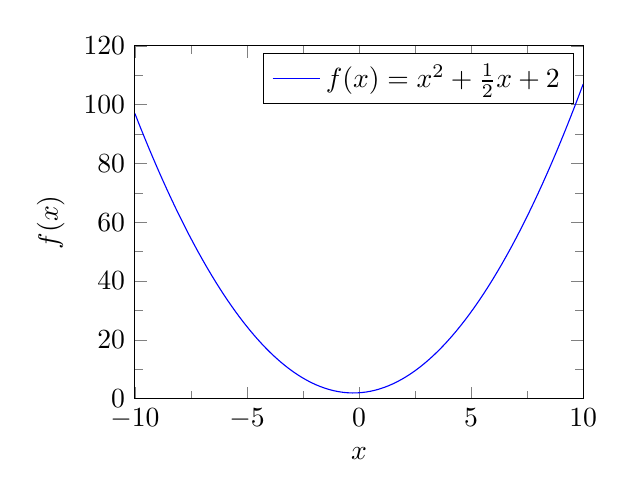
\begin{tikzpicture}
				\begin{axis}[
					width=.6\textwidth,
					height=.5\textwidth,
					domain=-10:10,
					xmin=-10, xmax=10,
					ymin=0, ymax=120,
					samples=100,
					ytick distance = 20,
					minor tick num = 1,
					%grid = both,
					%title = {\textbf{Parabelplot mit TikZ}},
					xlabel = {$x$},
					ylabel = {$f(x)$},
					legend entries = {$f(x) = x^2 + \frac{1}{2}x + 2$},
					]
					\addplot+[mark=none] {x^2 + 0.5*x + 2};
				\end{axis}
			\end{tikzpicture}
			\caption{Example plot for an expression using pgfplots}
			\label{fig:parabelpgf}
		\end{figure}
	
		Another, more advanced example is given in Figure~\ref{fig:sparameterpgf}. It uses a 2-port S-Parameter file to plot the input reflection in a smith chart and also reflection and transmission in a linear plot. The diagrams are created in a separate file using standalone. Also note that the package \texttt{subcaption} is used to create subplots.
	
		\begin{figure}[h]
			\centering
			\begin{subfigure}{0.75\textwidth}
				\centering
				\includestandalone{standalones/sparameter/sparameterSmith}
				\caption{Smith Chart plot}
			\end{subfigure}
			\\
			\begin{subfigure}{0.75\textwidth}
				\centering
				\includestandalone{standalones/sparameter/sparameter}
				\caption{}
			\end{subfigure}
			\caption{S-Parameter of a filter created on the website \url{https://rf-tools.com}}
			\label{fig:sparameterpgf}
		\end{figure}
		
		\subsubsection{Matlab plots}
		
		To avoid the use of pixel graphics there exist tools like \texttt{matlab2tikz}\footnote{\url{https://github.com/matlab2tikz/matlab2tikz}}. It is recommended to use such a tool to generate high quality plots with a consistent style. \texttt{matlab2tikz} works by generating a \texttt{tex} file from within Matlab. For detailed installation and usage it is referred to the given github repository and the Matlab FileExchange.
		
		A simple example is given below:
		
		\begin{lstlisting}[language=Matlab]
			% generate x and y data
			x=-10:0.1:10;
			y=x.^2 + 1/2*x + 2;
			
			% plotting
			figure(1);
			hold on;
			xlabel('$x$');
			ylabel('$f(x)$');
			plot(x,y,'r')
			legend('$f(x)=x^2 + \frac{1}{2}x + 2$');
			matlab2tikz('pathtotargetfile/matlabtikz.tikz', 'width', '0.5\textwidth', 'parseStrings', false);
		\end{lstlisting}
	
		When previewing graphs in Matlab axis labels appear corrupted because the {\LaTeX} commands are not interpreted in the preview due to the \texttt{parseStrings} option. 
		
		\subsubsection{Python plots using matplotlib}
		
		There are several possibilities to include python plots in {\LaTeX} documents. One of them is the \texttt{pgf} mode of \texttt{matplotlib}. It can be activated with \verb|mpl.use('pgf')| and finally the output can be saved with \verb|plt.savefig("pa2.pgf",bbox_inches='tight')| and \verb|plt.close()|. This method has the advantage that {\LaTeX} expressions inside the graphic are interpreted in the main document allowing i.e. to include cites.
		
		An alternative is \texttt{tikzplotlib} \footnote{\url{https://pypi.org/project/tikzplotlib/}} which allows a more consistent style.
		
	\subsection{Tables}
	
		There are several enhancements for {\LaTeX} tables to improve the default \texttt{tabular} environment. The \texttt{bama} class uses \texttt{longtable} for multi page tables and \texttt{booktabs} for a cleaner design. A simple example is given below:
		
		\begin{lstlisting}[language=TeX]
			\begin{table}
				\centering
				\caption{myTableCaption}
				\label{tab:myTable}
				\begin{longtable}{cc}
					\toprule
					header & second column\\
					\midrule
					content & second column\\
					next row & second column\\
					\bottomrule
				\end{longtable}
			\end{table}
		\end{lstlisting}
	
\section{Lists}

This section refers to lists like the table of contents, list of abbreviations, \dots. These are automatically generated by {\LaTeX}. In order to fully populate them several runs of the compiler may are necessary because the references have to be found in the current run but can not be processed until the next run.

The lists can be generated by the following commands. Some of them are modified by the template in order to provide the required style.

\begin{table}
	\centering
	\caption{Lists of a thesis}
	\label{tab:listofs}
	\begin{tabular}{ll}
		\toprule
		Table of contents:    & {\verb|\tableofcontents|} \\
		List of abbreviations: & {\verb|\printacronyms|} \\
		Bibliography:  & {\verb|\printbibliography|} \\
		List of figures: & {\verb|\listoffigures|} \\
		List of tables:   & {\verb|\listoftables|}\\
		\bottomrule
	\end{tabular}
\end{table}

	\subsection{Abbreviations}
	\label{sec:acronyms}

	Despite a lot of abbreviations are very common in science and engineering the long form of every abbreviation has to be included in the thesis. Therefore there is the package \texttt{acro} which offers the definition of abbreviations in separate file (\texttt{acronyms.tex}) and their use in the document.
	
	\begin{lstlisting}[language=TeX]
	\DeclareAcronym{MOSFET}{
		short = MOSFET,
		long  = Metal-Oxide-Semi\-conductor Field-Effect Tran\-sistor
	}
	\end{lstlisting}

	The abbreviation can be inserted with \verb|\ac{key}| This uses the long form at the first time like \ac{MOSFET} and the short form on the following uses like \ac{MOSFET}.
	
	Long and short forms can also be enforced using \verb|\acl| and \verb|\acs|. Beside that several commands for singular, plural, \dots are available.
	
	Used abbreviations are also included into the list of abbreviations.

	\subsection{Citations}
	\label{sec:literatur}

	Quote worthy literature is cited by the command \verb|\cite| with the literatures key as argument. The style is defined by the template and should by used for a thesis at \acs{LTE} which looks like \cite{BibDEMO1}. Cites can be inserted in the middle of sentences or at the end. Citations at the end of a sentence must be preluded by a space and directly followed by the full stop.
	
	The correct and complete citation of information from literature is absolutely mandatory. A good practice is to insert citations into the caption of figures if they are not created by the author. Referencing common knowledge like Ohm's Law is not necessary.
	
	Bibliography data is stored in bibfiles. There is an entry for every reference.
	
		\begin{verbatim}
		@Article{JassSenBigPaper,
   author  = {Hugh {Jass sen.}},
   title   = {A very-big paper},
   journal = {The journal of very big papers},
   year    = {7991},
   volume  = {MCMXCVII},
		}
		\end{verbatim}
		
		The entry is referred to by the key which is necessary for citing: \verb|\cite{JassSenBigPaper}|. Even before the key is the type of the publication like article, book, conference, online and much more. Additional information is stored according to the chosen type. Depending on the reference type the entry contains different information and looks different in the list of bibliography.
		
		Brackets are used in different places of the entry to avoid wrong wrong formatting. The example uses a bracket to declare \enquote{Jass sen.} as the last name. Otherwise {\LaTeX} would detect \enquote{sen.} as the last name which would lead to an incorrect entry in the list of bibliography.
		
		Luckily the entries rarely have to be created manually. For books the website of the university library\footnote{\url{https://ub.fau.de/}} can serve as a comprehensive source. The entries can also be obtained by the publisher. Citations for papers in electronics engineering can be mostly downloaded from \footnote{\url{https://ieeexplore.ieee.org/}}. To make the job even easier there are numerous tools for managing bibfiles. A common tool is JabRef \footnote{\url{https://www.jabref.org/}} which allows for direct imports from IEEExplore by their number. The automatic formatting generation of citekeys can also be handy. Furthermore JabRef supports the import of metadata from PDFs. Simple drag and drop can be used to import references into JabRef. The current bama template is setup to contain the necessary data.
		
		The entries should contain a unique identifier to yield a useful bibliography. This can be the ISBN for books like \cite{tietze2019} or the DOI for digital formats like \cite{paskin1999}. The corresponding url is automatically inserted as invisible link into the bibliography.
		
		Less scientific works can be described by the type \texttt{TechReport} or \texttt{online} like \cite{stm32l476, lehman2020}. These often do not contain a single author which is ok, but it has to be made sure that the reference can be found e.g. by giving a revision number.
		
		The inclusion of bibliography data is not done by {\LaTeX} itself but the a bibliography backend. In this template \texttt{biber} is used which generates a file that is included in additional runs of {\LaTeX}. This mechanism is the reason why several iterations are necessary to fully populate the bibliography.

	\section{Source Code}

		Code can be included by the environment \texttt{lstlisting}. Code can be directly inserted by the following command.
		
		\lstnewenvironment{lstlistingoflisting}
		{\lstset{language=TeX}}
		{}
		\begin{lstlistingoflisting}[language=TeX]
			\begin{lstlisting}[language=C]
				#include<stdio.h>
				
				int main(void) {
					printf("Hallo Welt"); // comment (Test for special chars: äöüß)
					return 0;
				}
			\end{lstlisting}
		\end{lstlistingoflisting}
	
		yielding

		\begin{lstlisting}[language=C]
			#include<stdio.h>

			int main(void) {
				printf("Hallo Welt"); // comment (Test for special chars: äöüß)
				return 0;
			}
  		\end{lstlisting}

		Code can also be read in form files with \texttt{firstline} and \texttt{lastline} specifying the used part of the file. \texttt{firstnumber} is the first number on the left side of the code block.
		
		\begin{lstlisting}[language=C]
			\lstinputlisting[language=C, firstline=15, lastline=17, firstnumber=15]{code/codeexample.c}
		 \end{lstlisting}
		
	\section{Indices\index{Indices}}
	
		{\LaTeX} also supports the creation of indices but it has been removed from the template due to the seldom use. It can be added with the package \texttt{imakeidx}. It supports simple indice \verb|\index{indice}| and sub-indices \verb|\index{indice!subindice}|. It is necessary to also execute \textit{makeindex} in a similar fashion than the bibliography.

	\section{Why Lua{\LaTeX}?}
	
		Lua{\LaTeX} supports additional features compared to pdflatex like direct entering of \enquote{°}, \enquote{µ} and umlaut in the code. It is also possible to execute scripts like outputting the value of $\pipi = \SI{\directlua{tex.print(math.pi)}}{}$ or the generation of PDF metadata from user variables.
		
	\section{Additional packages}
	
	Feel free to modify the files in the \texttt{header} folder to include further packages if you have additional needs like making notes with the \texttt{ToDoNotes} package which allows inserting colourful notes that can be hidden with one switch.
	
	If you have found an improvement to basic settings and packages please let the maintainer of the template know in order to improve the template.

\section{Troubleshooting}
\label{sec:troubleshooting}

	Aside from errors in the source code being one of the top reasons problems can also arise due to outdated files created by the {\LaTeX} Compiler. Deleting auxiliary files, by hand or with the function of TeXstudio, and recompiling the document can solve the problem. Further error sources are listed below.
	
	\begin{itemize}
		\item Outdated packages; {\LaTeX} packages are updated regularly. This can lead to outdated packages of the user which can be resolved by updating or the use of outdated options of the template.
		\item Missing packages; Wrong spelling of commands or using commands of not included packages lead to errors.
		\item Missing or wrong brackets
		\item Environments which do not end or are incorrectly nested.
		\item Using match commands like \verb|\frac| outside of the math mode.
		\item Tables spanning more than one page. This can resolved with the \texttt{longtable} package.
		\item Wrong format of source code files. \enquote{utf8} is recommended.
	\end{itemize}

	Further good practices are:
	\begin{itemize}
		\item Do not change files of the {\LaTeX}-installation. This avoids compilation on other machines.
		\item Do not use absolute paths. This avoids compiling the document on other machines.
	\end{itemize}

	For the most problems there is a lot of information available online. Common and also not that common problems can be found in forums but the package documentations are also pretty helpful.
